\documentclass{article}

% Language setting
% Replace `english' with e.g. `spanish' to change the document language
\usepackage[english]{babel}

\usepackage[final]{neurips2023}
\makeatletter
\renewcommand{\@noticestring}{}
\makeatother

% Useful packages
\usepackage{amsmath}
\usepackage{graphicx}
\usepackage[colorlinks=true, allcolors=blue]{hyperref}
\usepackage{amsfonts}
\usepackage{booktabs}
\usepackage{multirow}
\usepackage{multicol}

\usepackage{tikz}
\usetikzlibrary{shapes.geometric, arrows.meta, positioning, fit, backgrounds, calc, shadows}

\definecolor{colInput}{RGB}{230, 230, 230}
\definecolor{colHead}{RGB}{255, 242, 204}
\definecolor{colPred}{RGB}{218, 232, 252}
\definecolor{colAttn}{RGB}{213, 232, 212}
\definecolor{colNovel}{RGB}{245, 245, 245}
\definecolor{colLoss}{RGB}{255, 204, 204}
\definecolor{colContainerGray}{RGB}{242, 242, 242}
\definecolor{colContainerOrange}{RGB}{255, 235, 215}

\title{Transfer Learning Project}
\author{%
  Chenyu Tian \\
  Columbia University\\
  \texttt{ct3308@columbia.edu} \\
  \And
  Yilu Yang \\
  Columbia University\\
  \texttt{yy3626@columbia.edu}
}

\begin{document}
\maketitle

\section{Introduction}
This project aims to solve a hierarchical classification problem by predicting both a superclass and its corresponding subclass for a given image. The problem has two primary complexities that test model robustness and generalization:

\textbf{Open Set Recognition (OSR):} The test set contains novel superclasses and subclasses not seen (out-of-distribution samples) during training. The model must identify and reject these ``unknown'' samples as ``novel''.

\textbf{Distribution Shift:} The test set's class frequencies may differ from the training set. The model must generalize to this new statistical distribution of known classes.


\section{Related Work}
OSR contrasts with traditional closed-set recognition, which assumes all testing classes are known during training. The methods for solving OSR problems primarily fall into the following two groups~\cite{sun2023survey}.

\textbf{Discriminative Models:} Discriminative models aim to learn decision rules directly. This is often approached either by learning highly compact and discriminative representations for known classes (through score-based, distance-based or reconstruction-based methods) or by explicitly introducing "unknown" information into the training process. This unknown information can be synthesized from known classes.

\textbf{Generative Models:} The generative models is another approach which can be further divided into Instance and Non-Instance Generation-based methods~\cite{geng2020recent}. The former method focuses on generating useful new samples, while the second one focuses on learning the underlying distributions of the known-class data, often using Autoencoders (AEs) or Generative Adversarial Networks (GANs). The principle is that unknown samples will not fit the learned distributions, allowing for their detection based on deviation or high reconstruction error.


\section{Methods}
\subsection{Framework}

Since this is a hierarchical OSR problem, we propose different hierarchical models.

\begin{itemize}
    \item \textbf{Model Structure:} Use a pre-trained feature extractor (e.g., CLIP~\cite{radford2021learningtransferablevisualmodels}) followed by a superclass classification head and a subclass classification head, and train the network jointly using a combined loss from both heads.
    \item \textbf{Hierarchical Constraints:} To ensure the superclass classification impacts the subclass classification, we apply a \textbf{SE-style Feature Gating}~\cite{hu2019squeezeandexcitationnetworks}) soft constraint during training and a \textbf{Hierarchical Masking} hard constraint during inference.
\end{itemize}

\paragraph{Training with SE-style Feature Gating:}
During Training, we apply SE-style Feature Gating to recalibrate features based on their importance for superclass classification.

Given input features $\mathbf{x} \in \mathbb{R}^{d}$ from CLIP, we define:

\textit{Superclass Head:}
\begin{equation}
    \mathbf{z}^{\text{super}} = W^{\text{super}} \mathbf{x} + \mathbf{b}^{\text{super}}
\end{equation}

\textit{SE Feature Gating (Squeeze-Excitation):}
\begin{align}
    \mathbf{s} &= \sigma(W_2 \cdot \text{ReLU}(W_1 \mathbf{x})) \quad &\text{(Squeeze \& Excitation)} \\
    \tilde{\mathbf{x}} &= \mathbf{s} \odot \mathbf{x} \quad &\text{(Feature Recalibration)}
\end{align}
where $W_1 \in \mathbb{R}^{(d/r) \times d}$, $W_2 \in \mathbb{R}^{d \times (d/r)}$, $r=4$ is the reduction ratio, and $\odot$ denotes element-wise multiplication.

\textit{Subclass Head (with attended features):}
\begin{equation}
    \mathbf{z}^{\text{sub}} = W^{\text{sub}} \tilde{\mathbf{x}} + \mathbf{b}^{\text{sub}}
\end{equation}

\paragraph{Inference with Hierarchical Masking:}
During inference, we apply hierarchical masking to enforce consistency between superclass and subclass predictions.

\begin{equation}
    \tilde{z}^{\text{sub}}_i =
    \begin{cases}
        z^{\text{sub}}_i & \text{if } i \in \mathcal{S}_{\hat{c}^{\text{super}}} \\
        -\infty & \text{otherwise}
    \end{cases}
\end{equation}

\subsection{Post-hoc Methods}

\subsubsection{Threshold Calibration Methods}

To classify a sample $\mathbf{x}$ as known or novel, we define a scoring function $S(\mathbf{x})$ where higher values indicate higher confidence in known classes. The decision rule is defined as:
\begin{equation}
    \hat{y} =
    \begin{cases}
        \text{Known}, & \text{if } S(\mathbf{x}) \geq \tau \\
        \text{Novel}, & \text{if } S(\mathbf{x}) < \tau
    \end{cases}
\end{equation}
We explore three methods to determine the optimal threshold $\tau$, depending on the availability of novel samples in the validation set.

\paragraph{Quantile-based Threshold (Non-Parametric).}
Used in \textit{Strict Open-Set Calibration}. This method assumes no prior knowledge of the unknown distribution. Given a target recall rate $r$ (e.g., $r = 0.95$) for known classes, we set $\tau$ as the $(1-r)$-th quantile of the scores from the known validation set $\mathcal{D}_{\text{val}}^{\text{known}}$:
\begin{equation}
    \tau_{\text{Quantile}} = Q_{1-r}(\{S(\mathbf{x}) \mid \mathbf{x} \in \mathcal{D}_{\text{val}}^{\text{known}}\})
\end{equation}
This approach is distribution-free and guarantees that exactly $r$ fraction of known samples are retained, but it does not account for the density of novel samples.

\paragraph{Z-Score Threshold (Parametric).}
Also used in \textit{Strict Open-Set Calibration}. We assume the scores of known classes follow a Gaussian distribution $\mathcal{N}(\mu, \sigma^2)$. The threshold is determined by a standard deviation multiplier $k$:
\begin{equation}
    \tau_{\text{Z-Score}} = \mu - k \cdot \sigma
\end{equation}
where $\mu$ and $\sigma$ are the mean and standard deviation of $S(\mathbf{x})$ on $\mathcal{D}_{\text{val}}^{\text{known}}$. For a target recall of 95\% under a normal distribution, we set $k=1.645$. This method is generally more robust to sampling noise than the Quantile method, provided the score distribution is approximately normal, but may underperform on heavy-tailed distributions.

\paragraph{Equal Error Rate (EER) Threshold (Full Validation).}
Used in \textit{Guided Open-Set Calibration}. When the validation set contains both known and novel samples ($\mathcal{D}_{\text{val}}^{\text{known}} \cup \mathcal{D}_{\text{val}}^{\text{novel}}$), we can explicitly model the boundary between the two distributions. We calculate $\tau$ as the intersection point of the empirical distributions, effectively balancing the FPR and FNR:
\begin{equation}
    \tau_{\text{Intersect}} = \operatorname*{argmin}_{t} \left| P(S(\mathbf{x}) < t \mid \text{Known}) - P(S(\mathbf{x}) \geq t \mid \text{Novel}) \right|
\end{equation}
This method theoretically yields the optimal separation for the observed validation distribution but relies on the assumption that the validation novelties are representative of the test novelties.

\begin{figure}[htbp]
    \centering
    \resizebox{\textwidth}{!}{
    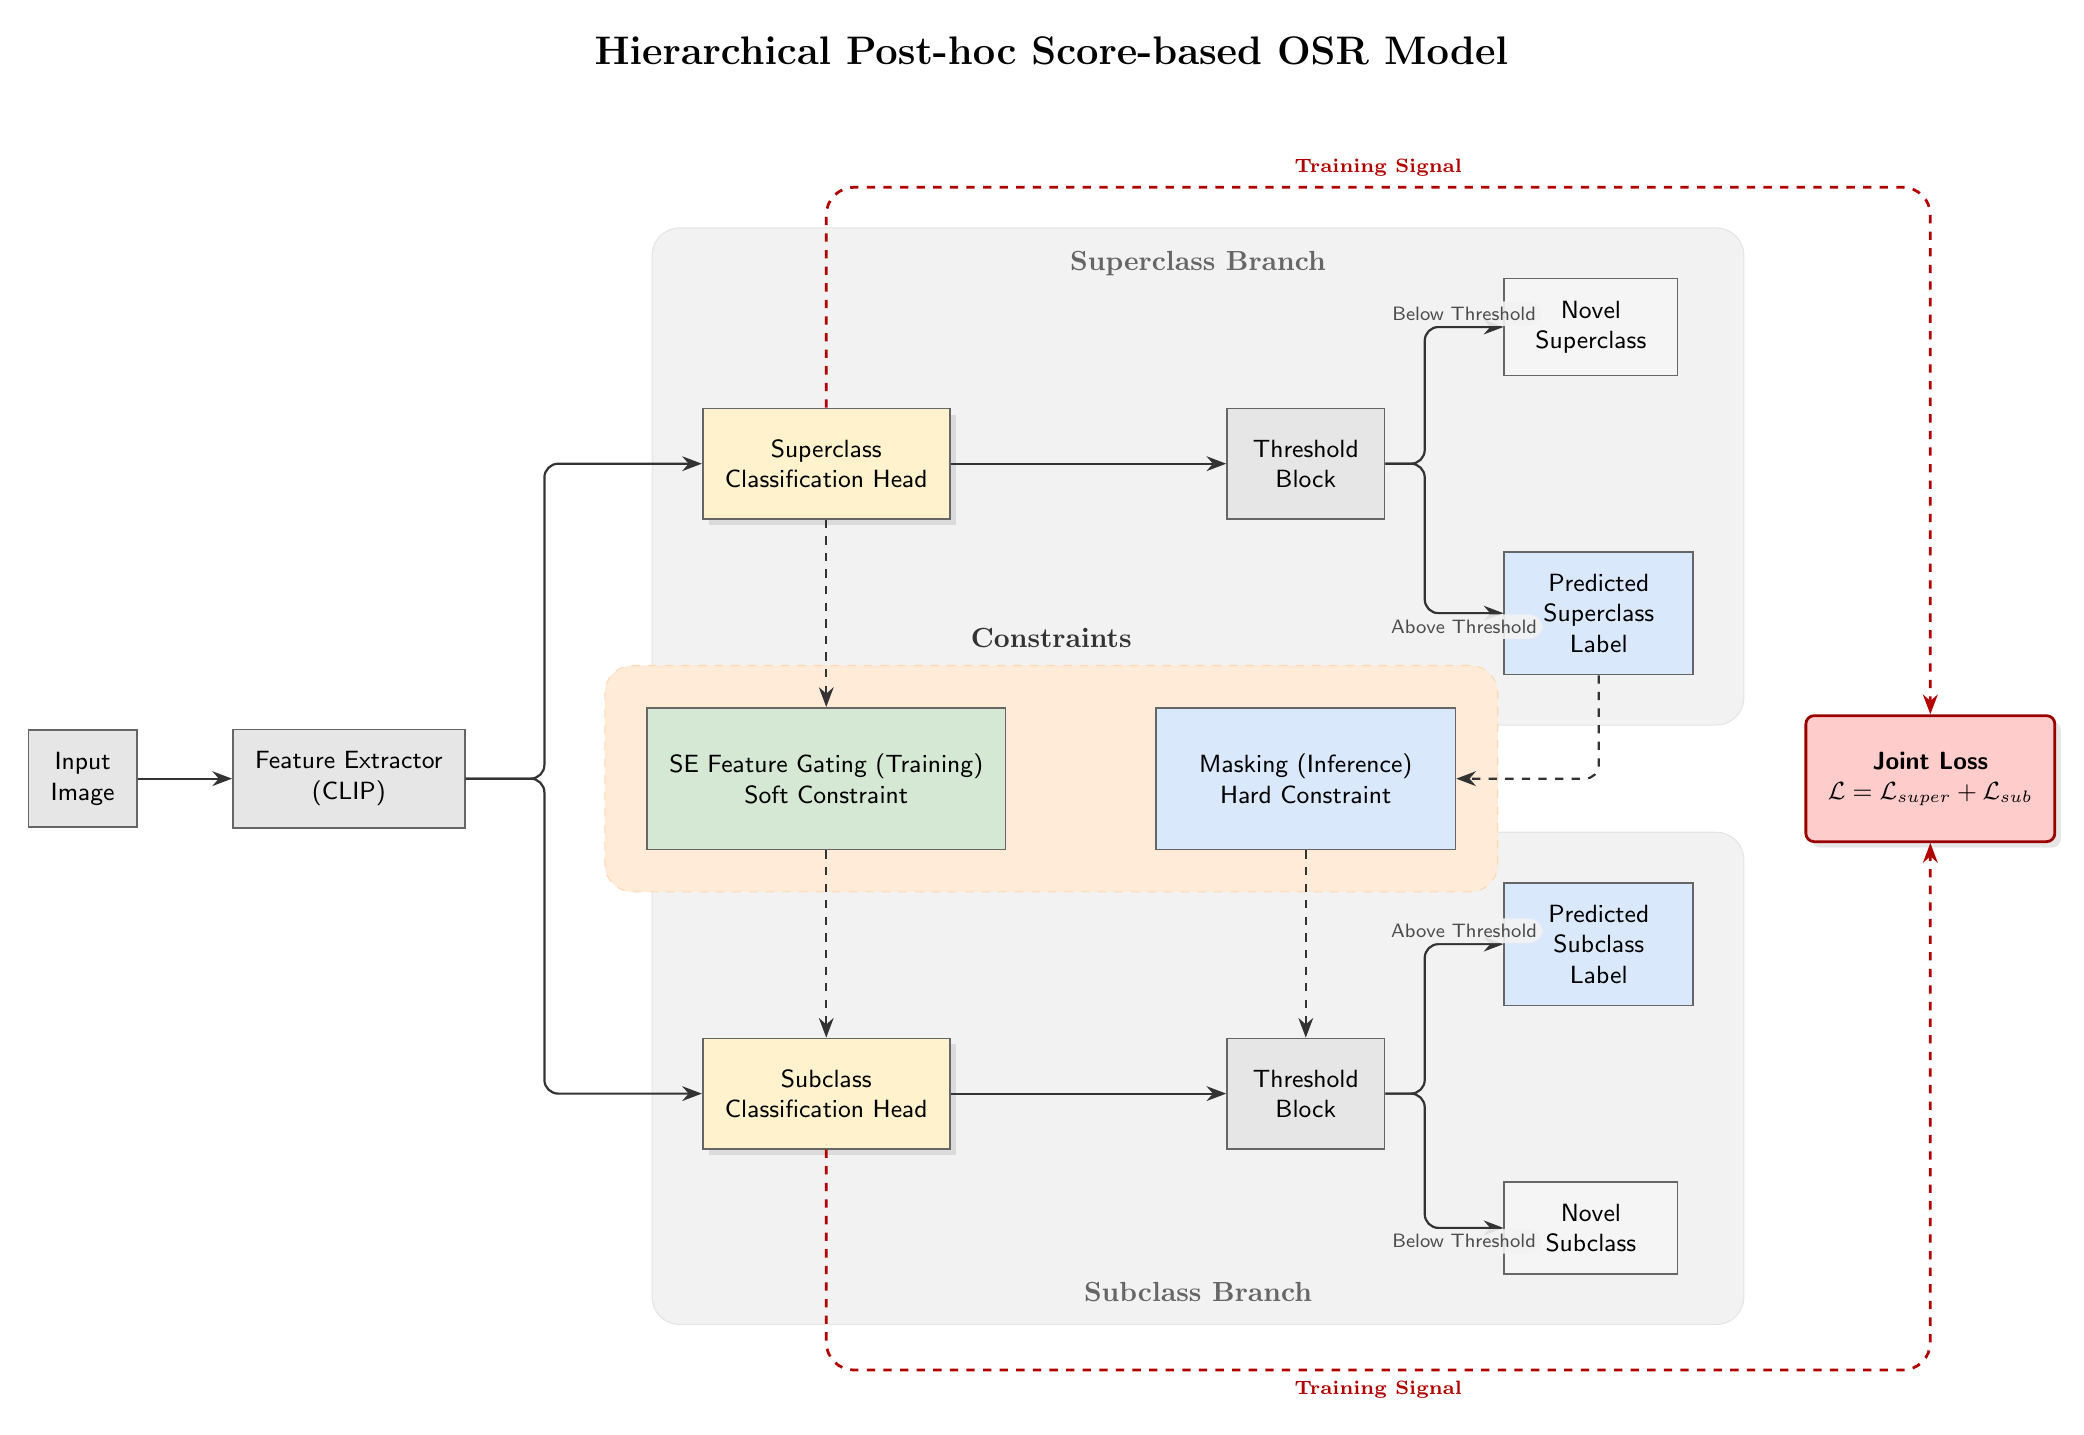
\begin{tikzpicture}[
        node distance=1.5cm and 2.2cm,
        font=\sffamily\small,
        >={Stealth[length=2.5mm]},
        % --- Node Styles ---
        base/.style={
            draw=black!60,
            rectangle,
            align=center,
            line width=0.6pt,
            inner sep=8pt
        },
        blockInput/.style={base, fill=colInput, minimum height=1.2cm},
        blockHead/.style={base, fill=colHead, minimum height=1.4cm, minimum width=2.8cm, drop shadow={opacity=0.2}},
        blockThresh/.style={base, fill=colInput, minimum height=1.4cm, minimum width=2.0cm},
        blockPred/.style={base, fill=colPred, minimum height=1.1cm, minimum width=2.4cm},
        blockNovel/.style={base, fill=colNovel, minimum height=0.9cm, minimum width=2.2cm},
        blockAttn/.style={base, fill=colAttn, minimum height=1.8cm, minimum width=3.8cm},
        blockMask/.style={base, fill=colPred, minimum height=1.8cm, minimum width=3.8cm},
        blockLoss/.style={base, fill=colLoss, minimum height=1.6cm, minimum width=2.5cm, rounded corners=3pt, drop shadow={opacity=0.2}, line width=1pt, draw=red!60!black},
        % --- Line Styles ---
        lineSolid/.style={->, draw=black!80, line width=0.8pt, rounded corners=5pt},
        lineDashed/.style={->, draw=black!80, dashed, line width=0.8pt, rounded corners=5pt},
        lineLoss/.style={->, draw=red!70!black, dashed, line width=1pt, rounded corners=10pt},
        labelSmall/.style={font=\scriptsize\sffamily, text=black!70, inner sep=2pt, fill=colContainerGray, fill opacity=0.9, text opacity=1}
    ]

        % ================= 1. Main Layout =================

        % Input
        \node[blockInput] (input) {Input\\Image};
        \node[blockInput, right=1.2cm of input] (extractor) {Feature Extractor\\(CLIP)};

        % --- Superclass Branch (Top) ---
        \node[blockHead, right=3.0cm of extractor, yshift=4.0cm] (super_head) {Superclass\\Classification Head};
        \node[blockThresh, right=3.5cm of super_head] (super_thresh) {Threshold\\Block};

        % Top Outputs (Novel above, Predicted below)
        \node[blockNovel, above right=0.4cm and 1.5cm of super_thresh] (super_novel) {Novel\\Superclass};
        \node[blockPred, below right=0.4cm and 1.5cm of super_thresh] (super_pred) {Predicted\\Superclass\\Label};

        % --- Subclass Branch (Bottom) - MIRRORED ---
        \node[blockHead, right=3.0cm of extractor, yshift=-4.0cm] (sub_head) {Subclass\\Classification Head};
        \node[blockThresh, right=3.5cm of sub_head] (sub_thresh) {Threshold\\Block};

        % Bottom Outputs - MIRRORED (Predicted above, Novel below)
        \node[blockPred, above right=0.4cm and 1.5cm of sub_thresh] (sub_pred) {Predicted\\Subclass\\Label};
        \node[blockNovel, below right=0.4cm and 1.5cm of sub_thresh] (sub_novel) {Novel\\Subclass};

        % --- Constraints (Middle) ---
        \node[blockAttn] at ($(super_head)!0.5!(sub_head)$) (attn) {SE Feature Gating (Training)\\Soft Constraint};
        \node[blockMask] at ($(super_thresh)!0.5!(sub_thresh)$) (mask) {Masking (Inference)\\Hard Constraint};

        % --- Joint Loss (Far Right) ---
        \node[blockLoss] at ($(super_pred.east)!0.5!(sub_pred.east) + (3, 0)$) (loss) {\textbf{Joint Loss}\\$\mathcal{L} = \mathcal{L}_{super} + \mathcal{L}_{sub}$};


        % ================= 2. Background Layer =================
        \begin{scope}[on background layer]
            % Superclass Container
            \node[fit=(super_head)(super_thresh)(super_novel)(super_pred),
                  fill=colContainerGray, draw=black!10, rounded corners=10pt, inner sep=18pt] (box_super) {};

            % Subclass Container
            \node[fit=(sub_head)(sub_thresh)(sub_novel)(sub_pred),
                  fill=colContainerGray, draw=black!10, rounded corners=10pt, inner sep=18pt] (box_sub) {};

            % Constraints Container
            \node[fit=(attn)(mask),
                  fill=colContainerOrange, draw=orange!30, dashed, rounded corners=10pt, inner sep=15pt] (box_constraints) {};
        \end{scope}

        % ================= 3. Labels =================

        % Superclass Label (at top)
        \node[anchor=north, font=\bfseries, text=black!60, xshift=0pt, yshift=-5pt]
            at (box_super.north) {Superclass Branch};

        % Subclass Label (at bottom)
        \node[anchor=south, font=\bfseries, text=black!60, xshift=0pt, yshift=5pt]
            at (box_sub.south) {Subclass Branch};

        % Title for constraints
        \node[above=0.1cm of box_constraints, font=\bfseries, text=black!80] {Constraints};


        % ================= 4. Connections =================

        % Input -> Extractor
        \draw[lineSolid] (input) -- (extractor);

        % Extractor -> Heads
        \draw[lineSolid] (extractor.east) -- ++(1.0,0) |- (super_head.west);
        \draw[lineSolid] (extractor.east) -- ++(1.0,0) |- (sub_head.west);

        % Heads -> Thresholds
        \draw[lineSolid] (super_head) -- (super_thresh);
        \draw[lineSolid] (sub_head) -- (sub_thresh);

        % Thresholds -> Outputs
        % Superclass (Novel above, Predicted below)
        \draw[lineSolid] (super_thresh.east) -- ++(0.5,0) |- (super_novel.west)
            node[pos=0.75, above, labelSmall] {Below Threshold};
        \draw[lineSolid] (super_thresh.east) -- ++(0.5,0) |- (super_pred.west)
            node[pos=0.75, below, labelSmall] {Above Threshold};

        % Subclass - MIRRORED (Predicted above, Novel below)
        \draw[lineSolid] (sub_thresh.east) -- ++(0.5,0) |- (sub_pred.west)
            node[pos=0.75, above, labelSmall] {Above Threshold};
        \draw[lineSolid] (sub_thresh.east) -- ++(0.5,0) |- (sub_novel.west)
            node[pos=0.75, below, labelSmall] {Below Threshold};


        % ================= 5. Dashed Constraint & Loss Flows =================

        % Attention Flow (symmetric)
        \draw[lineDashed] (super_head.south) -- (attn.north);
        \draw[lineDashed] (attn.south) -- (sub_head.north);

        % Masking Flow (symmetric)
        \draw[lineDashed] (super_pred.south) |- (mask.east);
        \draw[lineDashed] (mask.south) |- (sub_thresh.north);

        % --- Loss Flow (symmetric) ---

        % From Super Head -> Up -> Right -> Down -> Loss
        \draw[lineLoss] (super_head.north) -- ++(0, 2.8) -| (loss.north)
            node[pos=0.25, above, font=\scriptsize\bfseries, text=red!70!black] {Training Signal};

        % From Sub Head -> Down -> Right -> Up -> Loss (mirrored)
        \draw[lineLoss] (sub_head.south) -- ++(0, -2.8) -| (loss.south)
            node[pos=0.25, below, font=\scriptsize\bfseries, text=red!70!black] {Training Signal};

        % Main Title (Optional: You can remove this line if you prefer the Caption to be the only title)
        \node[above=7.5cm of box_constraints, font=\bfseries\Large] {Hierarchical Post-hoc Score-based OSR Model};

    \end{tikzpicture}
    }
    \caption{Hierarchical Post-hoc Score-based OSR Model Framework}
    \label{fig:framework}
\end{figure}

\subsubsection{Post-hoc Scoring with Softmax and CE Loss}

\paragraph{Threshold Scoring Methods:}
\begin{itemize}
    \item Maximum Softmax Probability (MSP)~\cite{hendrycks2018baselinedetectingmisclassifiedoutofdistribution}: The baseline approach. It uses the maximum value of the softmax distribution as the confidence score. Logit $\to$ Softmax $\to$ Threshold Gate.
    \item Out-of-Distribution Detector (ODIN)~\cite{liang2020enhancingreliabilityoutofdistributionimage}: Improves MSP by applying temperature scaling to the logits before softmax and adding small perturbations to the input image. Logit $\to$ Temperature Scaling $\to$ Softmax $\to$ Threshold Gate.
\end{itemize}

\paragraph{Maximum Softmax Probability (MSP) (with Temperature Scaling):}
The MSP score is defined as the maximum class probability:
\begin{equation}
    S_{\text{ODIN}}(\mathbf{x}; T) = \max_{i} \frac{\exp(z_i(\mathbf{x})/T)}{\sum_{j=1}^{C} \exp(z_j(\mathbf{x})/T)}
\end{equation}
\begin{equation}
    \lim_{T \to \infty} S_{\text{ODIN}}(\mathbf{x}; T) \approx \frac{1}{C} + \frac{1}{C \cdot T} \left( z_{\max}(\mathbf{x}) - \bar{z}(\mathbf{x}) \right)
\end{equation}
This reveals that high-temperature ODIN measures the \textbf{Relative Sharpness} of the logit distribution.

\paragraph{Magnitude Information:}
A known issue with MSP and ODIN is their reliance on the Softmax function. Softmax forces output probabilities to sum to 1, losing the magnitude information of the underlying logits. Logit-based scoring methods in the next part resolve this problem.

\subsubsection{Post-hoc Scoring with Sigmoid and BCE Loss}

\paragraph{Consistency between Threshold Scoring Method and Training Objective:}
While the MSP framework maintains consistency between its scoring method and the Cross-Entropy training objective (as both rely on normalized probabilities and discard magnitude), Logit-based OOD detection methods introduce a \textbf{theoretical inconsistency} by utilizing magnitude information that the standard Softmax-Cross-Entropy objective suppresses. To resolve this and explicitly preserve magnitude information for effective outlier detection, we replace the Softmax normalization with \textbf{class-wise Sigmoid activations} and adopt a \textbf{Binary Cross-Entropy (BCE)} loss. This formulation effectively treats the multi-class classification problem as a collection of independent \textbf{one-vs-rest (OvR)} binary tasks, ensuring that the training objective aligns with the magnitude-sensitive scoring functions~\cite{shu2017docdeepopenclassification}.

\paragraph{Threshold Scoring Methods}
\begin{itemize}
    \item Maximum Sigmoid (MaxSigmoid) Score~\cite{shu2017docdeepopenclassification}: Use the maximum value of the sigmoid distribution as the confidence score.
    \item Energy-based Out-of-distribution Detection~\cite{liu2021energybasedoutofdistributiondetection}: Uses the negative free energy derived from the logits as the scoring function.
\end{itemize}

\paragraph{Maximum Sigmoid (MaxSigmoid) Score (with Temperature Scaling):}
\begin{equation}
    S_{\text{MaxSigmoid}}(\mathbf{x}; T) = \max_{i} \sigma(z_i(\mathbf{x})/T)
\end{equation}

\paragraph{Energy Score (with Temperature Scaling):}
The energy score is defined as the negative free energy:
\begin{equation}
    S_{\text{Energy}}(\mathbf{x}; T) = -E(\mathbf{x}; T) = T \cdot \log \sum_{i=1}^{C} \exp(z_i(\mathbf{x})/T)
\end{equation}
Lower energy values indicate higher confidence that the sample belongs to a known class.

\begin{equation}
    \lim_{T \to 0} E(\mathbf{x}; T) = -\max_{i} z_i(\mathbf{x})
\end{equation}
This shows that low-temperature Energy reduces to the negative \textbf{MaxLogit}, measuring the \textbf{Absolute Magnitude} of the strongest prediction.

% ================================= Not going to Implement =================================
%\subsubsection{Trainable Confidence Estimation Methods}
%Unlike post-hoc methods, these approaches modify the model architecture during training to explicitly learn representations better suited for distinguishing known from unknown.
%
%\begin{itemize}
%    \item \textbf{Auxiliary Confidence Gating~\cite{devries2018learningconfidenceoutofdistributiondetection}:} Add a parallel confidence branch alongside the main classification branch. The network is trained to output both a class prediction and a scalar confidence score via a sigmoid output. The model learns to output low confidence for samples that are difficult to classify or likely out-of-distribution.
%\end{itemize}

\subsection{Adapted CAC Method}
Although post-hoc methods can address OSR without retraining the model, we postulate that distinguishing known from unknown samples requires more than applying post-hoc measures. To further address the OSR problem, we utilize the \textbf{Class Anchor Clustering (CAC)} framework~\cite{miller2021class}, a distance-based discriminative method rooted in metric learning.

In contrast, CAC explicitly regularizes the network to enforce strict intra-class compactness and maximize inter-class separability. Our adoption of CAC is further motivated by the semantic properties of the CLIP encoder. While CLIP’s contrastive pre-training naturally induces implicit clustering via cosine similarity, we employ CAC to rigorously map these semantic representations to a structured logit space where class centers are manually anchored to ensure maximal separation. By aligning the dense semantic clusters from CLIP with fixed, distinct anchors, we establish a robust feature space.

\begin{equation}
    \begin{gathered}
        \mathcal{L}_{\text{CAC}}(\mathbf{x}, y) = \mathcal{L}_{T}(\mathbf{x}, y) + \lambda \mathcal{L}_{A}(\mathbf{x}, y)\\
        \mathcal{L}_{T}(\mathbf{x}, y) = log(1+\sum_{j\neq y}^{N}e^{d_y - d_j})\\
        \mathcal{L}_{A}(\mathbf{x}, y) = \|f(\mathbf{x}-c_y)\|_2
    \end{gathered}
\end{equation}


To further enhance the discriminative power of the logit space, we also integrate the SE-attention mechanism in this part. By enabling the model to adaptively emphasize salient information within the CLIP image representations, this approach effectively enhance the performance in some setting.

\subsubsection{CAC-Negative}

In this project, we introduce two methodological improvements to the CAC paradigm, the first of which utilizes generated pseudo-outliers. To utilize the inherent sparsity of the logit space produced by CAC, our objective is to further provide explicit supervision regarding the spatial arrangement of non-class data. As equation \ref{eq:OpenMix_CAC_loss} shows, we extend the CAC loss function to include a regularization term that compresses negative samples towards the coordinate origin. This approach not only ensures that outliers are sequestered far from the known class anchors but also mitigates optimization instability by defining a clear embedding objective for the open space.

\begin{equation}
    \label{eq:OpenMix_CAC_loss}
    \begin{gathered}
        \mathcal{L}_{\text{CAC}}(\mathbf{x_{all}}, y_{all}) = \mathcal{L}_{T}(\mathbf{x}, y) + \lambda_A \mathcal{L}_{A}(\mathbf{x}, y) + \lambda_N \mathcal{L}_{N}(\mathbf{x'}) \\
        \mathcal{L}_{N}(\mathbf{x'}) = \|f(\mathbf{x'})\|_2
    \end{gathered}
\end{equation}

Where $\mathbf{x'}$ denotes the pseudo-samples synthesized via two distinct strategies: 1) self-mixing of rotated images, and 2) background extraction, obtained by removing the foreground object.


\subsubsection{CAC-OpenMax}
The second strategic adaptation involves the integration of OpenMax~\cite{7780542}, a post-hoc inference mechanism rooted in Extreme Value Theory (EVT), with the CAC framework. This combination is motivated by the topological structure enforced by CAC: under ideal training conditions, CAC minimizes intra-class variance, compelling known samples to concentrate tightly around their respective class anchors while pushing OOD samples to the periphery. Leveraging this optimized embedding space, OpenMax models the tail distribution of the distances using a Weibull distribution. This allows us to rigorously filter distributional outliers—samples located significantly far from any class prototype—thereby enhancing the model's capability to discriminate between seen and unseen categories.

\section{Experiment}

We evaluate the proposed models using CLIP ViT-B/32 features, and simulate the OSR scenario by setting some labels to be novel.

\textbf{Note on Metrics:} We focus our reporting on \textbf{Subclass} performance metrics. In our experimental setup, we did not introduce novel superclasses. However, since the Superclass and Subclass classification heads share the same underlying architecture and scoring mechanisms, the optimal methods identified for Subclasses are methodologically generalizable to the Superclass level.

\subsection{Dataset Preparation}

We implement three distinct data preparation strategies to simulate different experimental assumptions. It is achieved by partitioning the dataset into  \textit{Known} and \textit{Novel} categories, and holding out a specific ratio of subclasses to serve as the \textit{Novel} set.

\paragraph{Strict Open-Set Calibration:} \textit{Novel} samples appear only in the Test set.

This strategy simulates a strict scenario where no outliers are available during the development phase and is used in \textit{Post-hoc Method}. Thresholds must be determined using statistical methods based solely on the distribution of known data.

\paragraph{Guided Open-Set Calibration:} \textit{Novel} samples appear in the Test and Validation set.

This allows for calibrating thresholds by observing the known and unknown distributions and is used in \textit{Post-hoc Method}.

\paragraph{Open-Set Training with Synthesis:}
For discriminative training methods, we modify the training data preparation to include synthesized outliers. This is used in \textit{Training-time method}.
\begin{itemize}
    \item \textbf{Train:} Known classes + Synthesized Pseudo-outliers.
    \item \textbf{Val/Test:} Known + Real Novel classes.
\end{itemize}
Since real novel samples are inaccessible during training, we generate pseudo-outliers via data augmentation techniques (e.g., self-mixing, background extraction) to explicitly supervise the model in compacting the known class space.

\subsection{Ablation Study: Architecture and Thresholds}

Table \ref{tab:ablation} presents the ablation study starting from a Linear Dual Head baseline. The parametric \textbf{Z-Score} method significantly outperforms Quantile, implying Gaussian-like score distributions. \textbf{Temperature Scaling} further refines separation, while the \textbf{Gated Dual Head} achieves the best performance, validating that SE-Attention successfully enforces hierarchical constraints.

\begin{table}[h]
  \caption{Ablation study on model architecture and threshold strategies. (Metric: Subclass Performance)}
  \label{tab:ablation}
  \centering
  \resizebox{\columnwidth}{!}{
  \begin{tabular}{lccccc}
    \toprule
    \bf Model Configuration & \bf Threshold & \bf Overall Acc. & \bf Seen Acc. & \bf Unseen Acc. & \bf AUROC \\
    \midrule
    Linear Dual Head (Baseline) & Quantile & 65.22\% ± 0.51\% & 87.01\% ± 2.13\% & 43.53\% ± 2.55\% & 0.8540 ± 0.0283 \\
    Linear Dual Head & Z-Score & 69.99\% ± 2.43\% & \textbf{88.24\% ± 1.58\%} & 51.90\% ± 5.56\% & 0.8540 ± 0.0283 \\
    + Temperature ($T=1.5$) & Z-Score & 72.99\% ± 3.39\% & 87.33\% ± 1.59\% & 58.80\% ± 7.47\% & 0.8679 ± 0.0265 \\
    \textbf{+ Gated Dual Head (Ours)} & \textbf{Z-Score} & \textbf{73.83\% ± 3.88\%} & 88.03\% ± 1.30\% & \textbf{59.79\% ± 8.48\%} & \textbf{0.8821 ± 0.0234} \\
    \bottomrule
  \end{tabular}
  }
\end{table}

\subsection{Impact of Scoring Functions and Loss Objectives}

Table \ref{tab:scoring_comparison} compares different scoring functions. We employ \textbf{Z-Score} thresholds for the bounded probability-based methods (MSP, MaxSigmoid) and \textbf{Quantile} for the unbounded \textbf{Energy} scores.

The results indicate distinct trade-offs. \textbf{MaxSigmoid} achieves high overall accuracy but suffers from overconfidence, making it difficult to detect novel superclasses. \textbf{Energy} significantly degrades performance on known superclasses. Consequently, \textbf{CE + MSP} is selected as the optimal method, offering the most robust performance with the highest AUROC.

\begin{table}[h]
  \caption{Comparison of Scoring Functions and Training Objectives. (Model: Gated Dual Head)}
  \label{tab:scoring_comparison}
  \centering
  \resizebox{\columnwidth}{!}{
  \begin{tabular}{lccccc}
    \toprule
    \bf Method (Loss + Score) & \bf Temp ($T$) & \bf Overall Acc. & \bf Seen Acc. & \bf Unseen Acc. & \bf AUROC \\
    \midrule
    \textbf{CE + MSP} & 1.5 & 73.83\% ± 3.88\% & \textbf{88.03\% ± 1.30\%} & 59.79\% ± 8.48\% & \textbf{0.8821 ± 0.0234} \\
    \textbf{BCE + MaxSigmoid} & 0.2 & \textbf{75.30\% ± 3.70\%} & 87.29\% ± 0.84\% & \textbf{63.30\% ± 8.03\%} & 0.8721 ± 0.0365 \\
    BCE + Energy & 0.02 & 70.88\% ± 1.51\% & 87.29\% ± 0.89\% & 54.50\% ± 3.91\% & 0.8755 ± 0.0343 \\
    \bottomrule
  \end{tabular}
  }
\end{table}

\subsection{Impact of Calibration Strategy}

In the \textit{Strict} setting, thresholds are derived solely from known data (Z-Score). In the \textit{Guided} setting, the validation set includes unknown samples, allowing for the \textit{EER} method.

We employ a nested calibration protocol for rigorous evaluation: (1) an outer loop splits the full training set into train and test sets with novel subclasses reserved for test; (2) an inner loop further partitions the train set into sub-train and validation sets for threshold calibration; (3) thresholds are averaged across inner iterations, and the final model is retrained on the full train set before testing. This approach mirrors the real submission pipeline while avoiding data leakage.

As shown in Table~\ref{tab:val_strategy}, the Guided strategy with EER thresholding achieves superior performance, demonstrating that the distribution of validation outliers generalizes well to the test set.

\begin{table}[h]
  \caption{Impact of Calibration Strategy on Subclass Performance (Model: CE + MSP).}
  \label{tab:val_strategy}
  \centering
  \resizebox{\columnwidth}{!}{
  \begin{tabular}{lccccc}
    \toprule
    \bf Calibration Strategy & \bf Threshold Method & \bf Overall Acc. & \bf Seen Acc. & \bf Unseen Acc. & \bf AUROC \\
    \midrule
    Strict (Known Only) & Z-Score & 73.83\% ± 3.88\% & 88.03\% ± 1.30\% & 59.79\% ± 8.48\% & 0.8821 ± 0.0234 \\
    Guided (Quick Eval) & EER & 79.57\% ± 1.55\% & 72.68\% ± 2.61\% & 84.90\% ± 4.12\% & 0.8663 ± 0.0119 \\
    Guided + Nested Calibration & EER & \textbf{83.02\% ± 3.69\%} & \textbf{84.84\% ± 2.84\%} & \textbf{80.74\% ± 8.65\%} & \textbf{0.9117 ± 0.0318} \\
    \bottomrule
  \end{tabular}
  }
\end{table}


\subsection{Impact of Synthesized Pseudo samples on CAC}
Table \ref{tab: CAC VS. CAC-Negative} presents a comparative analysis between the origin CAC with SE-Attention and our proposed CAC-Negative. The empirical results demonstrate that CAC-Negative consistently outperforms CAC in terms of AUROC, overall accuracy and unseen accuracy, validating the efficacy of incorporating synthesized negative samples for Open Set Recognition.

\textbf{Synergy between SE-Attention and Negative Sampling:} While SE-Attention yields negligible gains for the sparse baseline CAC, it significantly improves CAC-Negative. This disparity stems from the topological characteristics of the embedding space: the introduction of pseudo-negative samples densifies the manifold, thereby enabling SE-Attention to capture meaningful dependencies and refine the decision boundary, which is otherwise ineffective in the sparse logit space of the original CAC.

\textbf{Inefficacy of Explicit Intra-class Clustering ($\lambda$):} Regarding the hyperparameter $\lambda$ (the weight for the loss of anchor clustering term), our experiments indicate that non-zero values deteriorate the performance of the original CAC and provide no substantial benefit to CAC-Negative. Consequently, we set $\lambda=0$. We attribute this to the relatively limited number of known categories (70 classes); simply maximizing inter-class separation appears sufficient for classification, rendering strict intra-class clustering constraints less critical.

\begin{table}[h]
  \caption{CAC VS. CAC-Negative.}
  \label{tab: CAC VS. CAC-Negative}
  \centering
  \resizebox{\columnwidth}{!}{
      \begin{tabular}{lcccc}
        \toprule
        \bf Parameter & \bf Overall Acc. & \bf Seen Acc. & \bf Unseen Acc. & \bf AUROC \\
        \midrule
        \multicolumn{5}{l}{CAC} \\
        \midrule
        $\lambda=0, Attn=0$ & 77.80\% ± 0.31\% & 85.49\% ± 0.35\% & 71.24\% ± 0.83\% & 0.8908 ± 0.0009\\
        $\lambda=0, Attn=4$ & 78.05\% ± 0.57\% & 85.76\% ± 0.36\% & 71.47\% ± 1.02\% & 0.8931 ± 0.0015\\
        $\lambda=0.1, Attn=4$ & 67.58\% ± 0.27\% & \textbf{86.27\% ± 0.67\%} & 51.64\% ± 0.99\% & 0.8237 ± 0.0031 \\
        \midrule
        \multicolumn{5}{l}{\textbf{CAC-Negative}} \\
        \midrule
        $\lambda_N=0.3, Attn=0$ & 76.84\% ± 0.46\% & 84.71\% ± 0.28\% & 70.13\% ± 0.92\% & 0.8978 ± 0.0025 \\
        $\lambda_N=0.3, Attn=4$ & 84.68\% ± 0.25\% & 77.49\% ± 0.99\% & 90.80\% ± 0.77\% & 0.9411 ± 0.0021 \\
        $\lambda_N=0.5, Attn=4$ & \textbf{86.17\% ± 0.30\%} & 77.45\% ± 0.43\% & \textbf{93.61\% ± 0.42\%} & \textbf{0.9526 ± 0.0027} \\
        \bottomrule
      \end{tabular}
  }
\end{table}

\subsection{Impact of Different Post-hoc Methods on CAC}

Table \ref{tab: CAC-post hoc} presents a comparative analysis of varying post-hoc inference mechanisms applied to the CAC framework, specifically benchmarking the threshold-based baseline against Z-Score and OpenMax.

\textbf{Performance of OpenMax:} Empirical results demonstrate that OpenMax yields the most superior performance, achieving an AUROC of 0.9281. Crucially, this method significantly boosts Unseen Accuracy (from 71.24\% to 88.46\%) while incurring only a marginal degradation in Seen Accuracy ($\approx 1\%$), indicating a robust trade-off between closed-set classification and open-set rejection.

\textbf{Inefficacy of Z-Score:} Conversely, Z-Score proves suboptimal, failing to outperform even the simple baseline. The method exhibits extreme sensitivity to $std\_m$, where slight increases cause Unseen Accuracy to collapse to zero. This confirms that the highly compact clusters induced by CAC render standard deviation-based metrics overly sensitive and ineffective compared to tail-based estimation.

\begin{table}[h]
  \caption{Post hoc methods on \textit{\textbf{CAC}}}
  \label{tab: CAC-post hoc}
  \centering
  \resizebox{\columnwidth}{!}{
      \begin{tabular}{lcccc}
        \toprule
        \bf Method & \bf Overall Acc. & \bf Seen Acc. & \bf Unseen Acc. & \bf AUROC \\
        \midrule
        threshold          & 77.80\% ± 0.31\% & \textbf{85.49\% ± 0.35\%} & 71.24\% ± 0.83\% & 0.8908 ± 0.0009\\
        Z-Score($std\_m=0.1$)          & 72.55\% ± 0.24\% & 81.06\% ± 0.29\% & 65.28\% ± 0.40\% & 0.8325 ± 0.0009 \\
        \textbf{OpenMax}($\lambda=0.1$)          & \textbf{86.62\% ± 0.16\%} & 84.47\% ± 0.38\% & \textbf{88.46\% ± 0.11\%} & \textbf{0.9281 ± 0.0026} \\
        \bottomrule
      \end{tabular}
  }
\end{table}

% \begin{table}[h]
%   \caption{Template}
%   \label{tab:complex_table}
%   \centering
%   \begin{tabular}{lcccc}
%     \toprule
%     \multirow{2}{*}{\bf Method} & \multicolumn{2}{c}{\bf Standard Metrics} & \multicolumn{2}{c}{\bf Advanced Metrics} \\
%     \cmidrule(r){2-3} \cmidrule(l){4-5}
%     & Acc@1 & Acc@5 & ECE & NLL \\
%     \midrule
%     Vanilla      & 76.5 & 92.1 & 0.15 & 1.20 \\
%     Mixup        & 77.9 & 93.5 & 0.10 & 0.98 \\
%     CutMix       & 78.2 & 93.8 & 0.09 & 0.95 \\
%     \bf Ours     & \bf 79.1 & \bf 94.5 & \bf 0.05 & \bf 0.85 \\
%     \bottomrule
%   \end{tabular}
% \end{table}

% \begin{table}[t]
%   \caption{Template}
%   \label{tab:wide_comparison}
%   \centering
%   % \small % 小一号字体
%   \begin{tabular}{lcccccccc}
%     \toprule
%     \multirow{2}{*}{\bf Parameter ($\lambda$)} & \multicolumn{4}{c}{\bf Baseline Model} & \multicolumn{4}{c}{\bf Our Model} \\
%     \cmidrule(lr){2-5} \cmidrule(lr){6-9}
%     & Acc. & Prec. & Rec. & F1 & Acc. & Prec. & Rec. & F1 \\
%     \midrule
%     Setting 1 ($\alpha=0.1$) & 85.1 & 84.2 & 83.5 & 83.8 & \bf 86.5 & \bf 85.8 & 84.2 & \bf 85.0 \\
%     Setting 2 ($\alpha=0.5$) & 86.2 & 85.0 & 84.1 & 84.5 & \bf 88.1 & \bf 87.2 & \bf 86.5 & \bf 86.8 \\
%     Setting 3 ($\alpha=0.9$) & 84.5 & 83.8 & 82.0 & 82.9 & \bf 87.0 & \bf 86.5 & \bf 85.0 & \bf 85.7 \\
%     \bottomrule
%   \end{tabular}
% \end{table}

\bibliographystyle{alpha}
\bibliography{reference}

\end{document}
